

 \setcounter{section}{4}
\section{Safety \& Sustainability}
\bigskip
\subsection{Safety}
\medskip
The Akriveia Beacon system is a combination of electronics, wireless communication, and software systems all functioning together to create a reliable solution. Since the system is designed for disaster related situations, safety is paramount. There are essentially two conditions the system would be under; an idle mode from day to day; and an emergency mode where the system is triggered to transmit location data during a real disaster situation.

\bigskip
During idle mode or normal day to day operations the ID tags would be worn much like an access card. As such, electronic components on the ID tags must agree to standardized safety measurements. During emergency mode, in a disaster situation, the beacons are turned on to transmit and receive data from the ID tags. As the associated ID tags will be transmitting ultra-wideband radio frequency both to and from the radio modules which will be worn by a person, the power frequency level must be within limits that are safe for human exposure \cite{R22}.
 
\bigskip
Additionally, the Akriveia Beacon system will satisfy the following safety requirements:

\bgroup
\def\arraystretch{1.5}
\begin{table}[H]
\centering
\begin{tabular}{ | m{3cm} | m{13cm}| } 
\hline
\textbf{REQ.SF.1 - F} & All 2.4 GHz transceiver must operate at a safe transmitting power level\\
\hline
\textbf{REQ.SF.2 - F} &  All UWB GHz transceiver must operate at a safe transmitting power level\\
\hline
\textbf{REQ.SF.3 - F} & All electrical components of the system must be electrically insulated \\
\hline
\textbf{REQ.SF.4 - F} & The ID tags must not cause minor ergonomic issues such as pinches or discomfort on the wearer.\\
\hline
\textbf{REQ.SF.5 - F} & The ID tags must not cause major safety issues such as shocks, burns, or lacerations on the wearer\\
\hline
\textbf{REQ.SF.6 - F} & The Beacons must have proper labeling on electrical components detailing safety and standards \\
\hline
\textbf{REQ.SF.7 - F} & The Beacon casing must have fire resistant shielding \\
\hline
\textbf{REQ.SF.8 - F} & The data processing unit must have a fire resistant shielding \\
\hline
\end{tabular}
\caption{Safety Requirements}
\end{table}	

\break
\subsection{Sustainability}
\medskip
The engineers at TRIWAVE SYSTEMS is committed to ensuring the final products is not only functionally effective, but also in compliance with the best environmental sustainability practices. As such, TRIWAVE SYSTEMS will be dedicated to minimizing impact of the environment by making design choices that are environmentally sustainable by following the Cradle to Cradle (\Gls{C2C}) standards. C2C refers to the process of development where all components used in manufacturing are able to be brought back into the development cycle \cite{R23}. By following the C2C Certified standards shown below \cite{R25}, the Akriveia Beacon system can be re-purposed or recycled as shown below in the figure by EPEA.

\begin{figure}[H]
\centering
    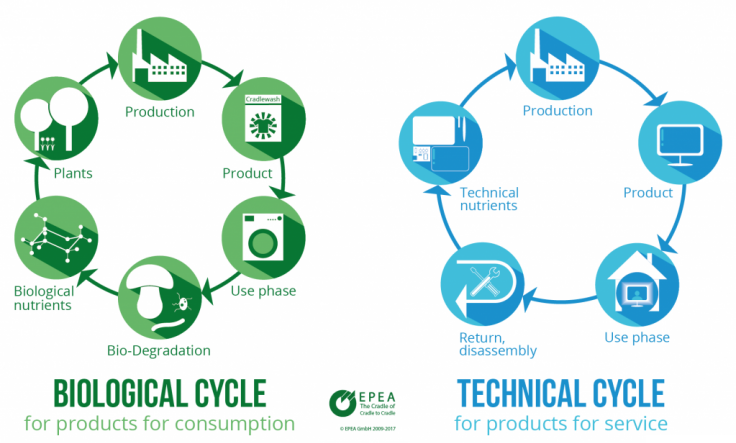
\includegraphics[scale=0.85]{./images/BioTechCycle.png}
    \caption{Biological and Technical C2C cycles}
\end{figure}

When possible, the Akriveia Beacon will be manufactured with biodegradable and non-toxic materials, as well as materials that are easily recyclable or re-purposable to ensure waste output is minimal. The material of choice for beacons and ID tag casings will be biodegradable non-toxic Polylactic acid or PLA plastics \cite{R25}. PLA is a natural, bio based alternative to petroleum laden ABS and used commonly in 3D printing processes. Electronics and circuitry of the product will be designed with a minimal footprint. Power sustainability is also considered by incorporating the use of RF harvesting. By converting radio frequency power into DC voltage to power devices, the need for constant battery replacement is minimized lowering maintenance costs. The following table includes the sustainability requirements for the system.

\break
The following table includes the sustainability requirements for the Akriveia Beacon system:

\bgroup
\def\arraystretch{1.5}
\begin{table}[H]
\centering
\begin{tabular}{ | m{3cm} | m{13cm}| } 
\hline
\textbf{REQ.SU.1 - F} & The ID tags must not need battery replacement within 1 year \\
\hline
\textbf{REQ.SU.2 - F} & The ID tags must use rechargeable batteries as a power source \\
\hline
\textbf{REQ.SU.3 - F} & The PCB for ID and Beacons must be no larger than 25mm x 60mm area \\
\hline
\textbf{REQ.SU.4 - F} & The ID tags will be no larger than 70mm x 140mm x 15mm \\
\hline
\textbf{REQ.SU.5 - F} & The ID tags must have removable casing manufactured with PLA plastic \\
\hline
\textbf{REQ.SU.6 - F} & The Beacons must have removable casing manufactured with PLA plastic \\
\hline
\textbf{REQ.SU.7 - F} & The electrical components within the ID tag or beacon devices must not need replacement within 1 year \\ 
\hline
\end{tabular}
\caption{Sustainability Requirements}
\end{table}	


%\end{document}